% !TEX program = lualatex
\documentclass[12pt,a4paper]{article}
\usepackage{graphicx}
\usepackage{fontspec}
\setmonofont{Latin Modern Mono}
\usepackage{xcolor}
\usepackage{listings}
\usepackage{geometry}
\usepackage{fancyhdr}
\usepackage{hyperref}
\usepackage{booktabs} 
\usepackage{float}    
\usepackage{amsmath}

% =======================================================
%  USER CONFIGURATION (EDIT VARIABLES HERE)
% =======================================================
\newcommand{\labNo}{Lab 9}
\newcommand{\labTopic}{JDBC with PostgreSQL}
\newcommand{\courseCode}{CSE 4308}
\newcommand{\courseTitleShort}{DBMS Lab}
\newcommand{\courseTitleLong}{DATABASE MANAGEMENT SYSTEMS LAB}
\newcommand{\instructorName}{Samnun Azfar, Jr. Lecturer, CSE\\ Samia Nawsheen, Jr. Lecturer, CSE}
\newcommand{\academicYear}{AY25-26}
% =======================================================

\geometry{margin=1in}

% -
% Header and Footer Configuration
% -
\pagestyle{fancy}
\fancyhf{}
\lhead{\labNo}                        % Uses variable
\rhead{\courseCode: \courseTitleShort} % Uses variables

% Centered footer with page number
\cfoot{\thepage}
% Ensure header/footer width matches text block
\setlength{\headwidth}{\textwidth}

% -
% Code Listing Style
% -
\definecolor{codegreen}{rgb}{0,0.6,0}
\definecolor{codegray}{rgb}{0.5,0.5,0.5}
\definecolor{codepurple}{rgb}{0.58,0,0.82}
\definecolor{backcolour}{rgb}{0.95,0.95,0.92}

\lstdefinestyle{mystyle}{
    backgroundcolor=\color{backcolour},
    commentstyle=\color{codegreen},
    keywordstyle=\color{magenta},
    numberstyle=\tiny\color{codegray},
    stringstyle=\color{codepurple},
    basicstyle=\ttfamily\footnotesize,
    breaklines=true,
    captionpos=b,
    keepspaces=true,
    numbers=left,
    numbersep=5pt,
    tabsize=2,
    frame=single,
    numbers=none,
    columns=fullflexible,
    showspaces=false,
    showstringspaces=false,
    showtabs=false,
}

\lstset{style=mystyle}

% Images: found next to this file (local compile_labs.sh) or via the
% lab folder when compiled from the project root (Overleaf).
\graphicspath{{lab_09_jdbc/}}

\begin{document}

% --
% TITLE PAGE
% --
\begin{titlepage}
    \centering
    \vspace*{2\baselineskip}

    \rule{14cm}{2pt}\vspace*{-0.8\baselineskip}\vspace*{1.5pt}
    \rule{14cm}{0.5pt}\vspace{2\baselineskip}

    {\Huge\bfseries\scshape \labNo\par} % Uses variable
    \vspace{3mm}
    {\Large \labTopic} % Uses variable
    \vspace{3mm}

    \rule{14cm}{0.5pt}\vspace*{-0.7\baselineskip}\vspace{2.5pt}
    \rule{14cm}{2pt}

    \vspace{2\baselineskip}

    {\Large\bfseries \courseCode\par} % Uses variable
    \vspace{1\baselineskip}
    {\large \courseTitleLong\par} % Uses variable

    \vfill
    {\normalsize Prepared by:\\ \instructorName\par} % Uses variable
    {\normalsize Academic Year: \academicYear\par} % Uses variable
\end{titlepage}

\newpage
\tableofcontents
\newpage

% =======================================================
% SECTION: LAB WORKFLOW
% =======================================================
\section{Lab Workflow}



\textit{Repeat this subsection for every single lab.}

\begin{enumerate}
\item Connect to the internet by running nmtui in terminal, add a dsl connection, then go back and activate that dsl connection. Make sure that your net id is not being used in any other pc or router, if you face any issue, use any other net id from your friends which is not being used.

\item Download all the files posted in the google classroom.

\item Disconnect from the \textbf{dsl} connection via nmtui, connect to the ethernet/wired connection via nmtui. If no such connection exists, create an \textbf{ethernet} connection  and then activate.

    \item \textbf{Create Your Role and Database}

Inside the PostgreSQL shell, create your own role (user) and database.

1. In the Linux terminal:
\begin{lstlisting}[language=bash]
psql
\end{lstlisting}

Expected prompt:
\begin{lstlisting}
cse=#
\end{lstlisting}

2. Create Your Role and Database

Copy and run the following commands inside PostgreSQL:
\begin{lstlisting}[language=SQL]
-- 1. Terminate existing database connections
SELECT pg_terminate_backend(pid)
FROM pg_stat_activity
WHERE datname = 'cse4308_12345'
  AND pid <> pg_backend_pid();

-- 2. Remove existing database
DROP DATABASE IF EXISTS cse4308_12345;

-- 3. Remove existing role
DROP ROLE IF EXISTS student_12345;

-- 4. Create role
CREATE ROLE student_12345 LOGIN;

-- 5. Set password
ALTER ROLE student_12345
WITH PASSWORD 'student12345';

-- 6. Create database
CREATE DATABASE cse4308_12345
OWNER student_12345;

-- 7. Grant privileges
GRANT ALL PRIVILEGES
ON DATABASE cse4308_12345
TO student_12345;
\end{lstlisting}

3. Exit PostgreSQL:

   \begin{lstlisting}[language=SQL]
   \q
   \end{lstlisting}

\item \textbf{Connect Using Your Newly Created User}

1. Connect to Your Database:

   Use the following command to log in as the \texttt{student\_12345} user:

   \begin{lstlisting}[language=SQL]
   psql -h localhost -U student_12345 -d cse4308_12345
   \end{lstlisting}

2. Verify the Connection:

   Verify that you are connected to the correct database with the following command:

   \begin{lstlisting}[language=SQL]
   \conninfo
   \end{lstlisting}

   Expected output:

   \begin{lstlisting}
   Database: cse4308_12345, User: student_12345
   \end{lstlisting}

3. Exit PostgreSQL:

   \begin{lstlisting}[language=SQL]
   \q
   \end{lstlisting}

\item \textbf{Load the Lab SQL File (MUST be run outside psql)}

Load the SQL file that sets up the tables and inserts initial data.

1. Load the SQL File:

   Run the following command to load the lab SQL file:

   \begin{lstlisting}[language=SQL]
   psql -h localhost -U student_12345 -d cse4308_12345 -f /home/cse/Downloads/lab_09_setup.sql
   \end{lstlisting}

   This will:
   - Drop old tables (if they exist).
   - Create new tables.
   - Insert initial rows of data.

\item \textbf{Reconnect and Verify Tables}

After loading the SQL file, reconnect to PostgreSQL to verify that the tables have been created.

1. Reconnect to Your Database:

   \begin{lstlisting}[language=SQL]
   psql -h localhost -U student_12345 -d cse4308_12345
   \end{lstlisting}

2. Check Tables:

   Verify the tables have been created by listing them:

   \begin{lstlisting}[language=SQL]
   \dt
   \end{lstlisting}

3. View Table Data:

   Verify the data by running the following SQL queries:

   \begin{lstlisting}[language=SQL]
   SELECT * FROM <table_name>;
   \end{lstlisting}

\item Open a text editor and save it in the appropriate submission name format \\ \texttt{fullid\_CSE4308\_L9\_T1.sql}. You will use this text editor to write your solutions, make sure to save it after writing each solution. The structure of this file will be:
\begin{lstlisting}[language=SQL]
-- Task 1
INSERT INTO students (student_id, name, major, gpa)
VALUES (104, 'David', 'ME', 3.60);
--Task 2
SELECT name, gpa FROM students WHERE major = 'CSE';
\end{lstlisting}
\end{enumerate}

% =======================================================
% SECTION: DATABASE SCHEMA & DATA
% =======================================================
\section{Database Schema \& Data File}
\textbf{Instructions:} Copy the code below and save it as a file named \texttt{lab\_09\_setup.sql} in your \texttt{Downloads} directory. This file will be used in Step 6 of the Lab Workflow.

\begin{lstlisting}[language=SQL, caption={lab\_09\_setup.sql}]
-- 1. CLEANUP
DROP TABLE IF EXISTS TRANSACTIONS;
DROP TABLE IF EXISTS ACCOUNT;

-- 2. CREATE TABLES
CREATE TABLE ACCOUNT (
    A_ID INT PRIMARY KEY
);

CREATE TABLE TRANSACTIONS (
    T_ID INT GENERATED BY DEFAULT AS IDENTITY PRIMARY KEY,
    DTM TIMESTAMP,
    A_ID INT,
    AMOUNT DECIMAL(15,2),
    TYPE INT, -- 0 for Credit, 1 for Debit
    FOREIGN KEY (A_ID) REFERENCES ACCOUNT(A_ID)
);

-- 3. INSERT ACCOUNTS (Generates 100 Accounts)
INSERT INTO ACCOUNT (A_ID)
SELECT generate_series(1, 100);

-- 4. INSERT TRANSACTIONS (Generates ~1000 random transactions)
INSERT INTO TRANSACTIONS (DTM, A_ID, AMOUNT, TYPE)
SELECT
    timestamp '2020-01-01' + 
    random() * (timestamp '2022-12-31' - timestamp '2020-01-01'),
    floor(random() * 100 + 1)::int,
    (random() * 990000 + 10000)::decimal(15,2),
    floor(random() * 2)::int
FROM generate_series(1, 1000); 

COMMIT;
\end{lstlisting}

% =======================================================
% SECTION: SYSTEM SETUP
% =======================================================
\newpage
\section{Environment Setup}

Since this lab involves Java Database Connectivity (JDBC), additional setup is required beyond the standard PostgreSQL workflow.

\subsection{System Installation}
Open your terminal (\texttt{Ctrl+Alt+T}) and run the following commands to install the JDK and PostgreSQL (if not already installed):

\begin{lstlisting}[language=bash]
# Update package list
sudo apt update

# Install default Java JDK
sudo apt install default-jdk

# Install PostgreSQL
sudo apt install postgresql postgresql-contrib

# Install VS Code (if not installed)
sudo snap install code --classic
\end{lstlisting}

\subsection{VS Code Configuration}
\begin{enumerate}
    \item \textbf{Install Java Extensions:}
    \begin{itemize}
        \item Open VS Code.
        \item Click on the Extensions icon (box icon on the left sidebar).
        \item Search for \textbf{"Extension Pack for Java"} by Microsoft and click Install.
    \end{itemize}

    \item \textbf{Get the PostgreSQL JDBC Driver:}
    \begin{itemize}
        \item Download the driver JAR file from: \url{https://jdbc.postgresql.org/download/}
        \item Save \texttt{postgresql-42.x.x.jar} to a known location (e.g., \texttt{Downloads}).
    \end{itemize}

    \item \textbf{Create Project \& Add Driver:}
    \begin{itemize}
        \item Press \texttt{Ctrl+Shift+P} $\rightarrow$ \texttt{Java: Create Java Project} $\rightarrow$ \texttt{No Build Tools}.
        \item In the \textbf{Java Projects} view (bottom-left sidebar), find \textbf{Referenced Libraries}.
        \item Click the \textbf{+} icon and select the \texttt{postgresql-42.x.x.jar} file you downloaded.
    \end{itemize}
\end{enumerate}

% =======================================================
% SECTION: UNDERSTANDING JDBC
% =======================================================
\newpage
\section{Understanding JDBC}

\subsection{What is JDBC?}
JDBC stands for \textbf{Java Database Connectivity}. It is a standard Java API (Application Programming Interface) that allows Java applications to interact with relational databases. Before JDBC, writing database applications was difficult because different databases (like PostgreSQL, MySQL, Oracle) used different proprietary APIs. JDBC provides a uniform interface, meaning you can write one piece of Java code and, by simply changing the "Driver", connect it to any supported database.

\subsection{How It Works: The Architecture}
The JDBC architecture consists of three main layers working together:

\begin{enumerate}
    \item \textbf{The Java Application (Your Code):}
    This is the code you write in VS Code. It uses standard Java classes like \texttt{Connection}, \texttt{Statement}, and \texttt{ResultSet}. Importantly, your code does not know the details of how PostgreSQL works internally; it only knows standard Java commands.

    \item \textbf{The JDBC Driver (The Translator):}
    This is the \texttt{.jar} file you downloaded (e.g., \texttt{postgresql-42.x.x.jar}). It acts as a bridge or translator. When your Java code says "Execute Query", the Driver translates that generic request into the specific network protocol that the PostgreSQL server understands.

    \item \textbf{The Database (PostgreSQL):}
    The actual storage engine running on your Ubuntu machine. It receives commands from the Driver, executes them, and returns data.
\end{enumerate}

\subsection{Core Components \& Syntax}
To connect to a database, you generally follow these 4 steps, which correspond to specific Java classes:

\begin{enumerate}
    \item \textbf{Load the Driver:} \texttt{Class.forName("org.postgresql.Driver");}
    \item \textbf{Establish Connection:} \texttt{DriverManager.getConnection(url, user, pass);}
    \item \textbf{Create Statement:} \texttt{con.createStatement();}
    \item \textbf{Execute \& Process:} \texttt{stmt.executeQuery(sql);}
\end{enumerate}

\subsection{Prepared Statements}
The \texttt{Statement} interface is sufficient for simple, static queries (like \texttt{SELECT * FROM table}). However, when your application needs to handle User Input (e.g., a user typing their ID to login), you must use a \texttt{PreparedStatement}.

\textbf{Why use PreparedStatement?}
\begin{enumerate}
    \item \textbf{Security (SQL Injection Prevention):} If you simply concatenate strings (e.g., \texttt{"SELECT * FROM users WHERE name = " + input}), a malicious user can type code instead of a name to hack your database. \texttt{PreparedStatement} treats all user input strictly as data, never as executable code.
    \item \textbf{Performance:} The database pre-compiles the SQL query structure once, making it faster to execute multiple times with different values.
\end{enumerate}

\subsection{Real-Life Application}
In a real-world scenario, such as an ATM machine:
\begin{itemize}
    \item When you insert your card (User Input), the Java application reads the card number.
    \item It uses JDBC to send a secure \texttt{SELECT pin FROM users WHERE card\_id = ?} query to the bank's database using a PreparedStatement.
    \item The database returns the result, and the Java app compares it to the PIN you entered.
\end{itemize}

% =======================================================
% SECTION: CODE EXAMPLES
% =======================================================
\newpage
\section{JDBC Code Examples}

\subsection{Basic Select (Using Statement)}
This code demonstrates how to connect to the database and execute a simple, static query.

\begin{lstlisting}[language=Java, caption={Reading Data (SELECT)}]
import java.sql.*;

public class Main {
    public static void main(String[] args) {
        String url = "jdbc:postgresql://localhost:5432/cse4308_12345";
        String username = "student_12345";
        String password = "student12345";

        try {
            Class.forName("org.postgresql.Driver");
            Connection con = DriverManager.getConnection(url, username, password);
            System.out.println("Connected!");

            Statement statement = con.createStatement();
            ResultSet result = statement.executeQuery("SELECT * FROM account LIMIT 5");

            while (result.next()) {
                System.out.println("Account ID: " + result.getInt("a_id"));
            }

            con.close();
        } catch (Exception e) {
            e.printStackTrace();
        }
    }
}
\end{lstlisting}

\subsection{How to Run the Code}
\textbf{Method 1: VS Code (Recommended)} \\
If you added the JAR file to "Referenced Libraries", click the \textbf{Run} button above \texttt{main}.

\textbf{Method 2: Terminal Command (Manual)}
\begin{lstlisting}[language=bash]
# Compile
javac -cp .:postgresql-42.7.3.jar Main.java
# Run
java -cp .:postgresql-42.7.3.jar Main
\end{lstlisting}

% =======================================================
% SECTION: TASKS
% =======================================================
\newpage
\section{Scenario}
Consider the (partial) schema of a Banking Management System.
\begin{itemize}
    \item \textbf{ACCOUNT} table: Contains only the account ID.
    \item \textbf{TRANSACTIONS} table: Stores transaction ID, date, account involved, amount, and type.
    \item \textbf{TYPE} column: $0$ for credit (add money), $1$ for debit (subtract money).
\end{itemize}

\begin{figure}[h]
    \centering
    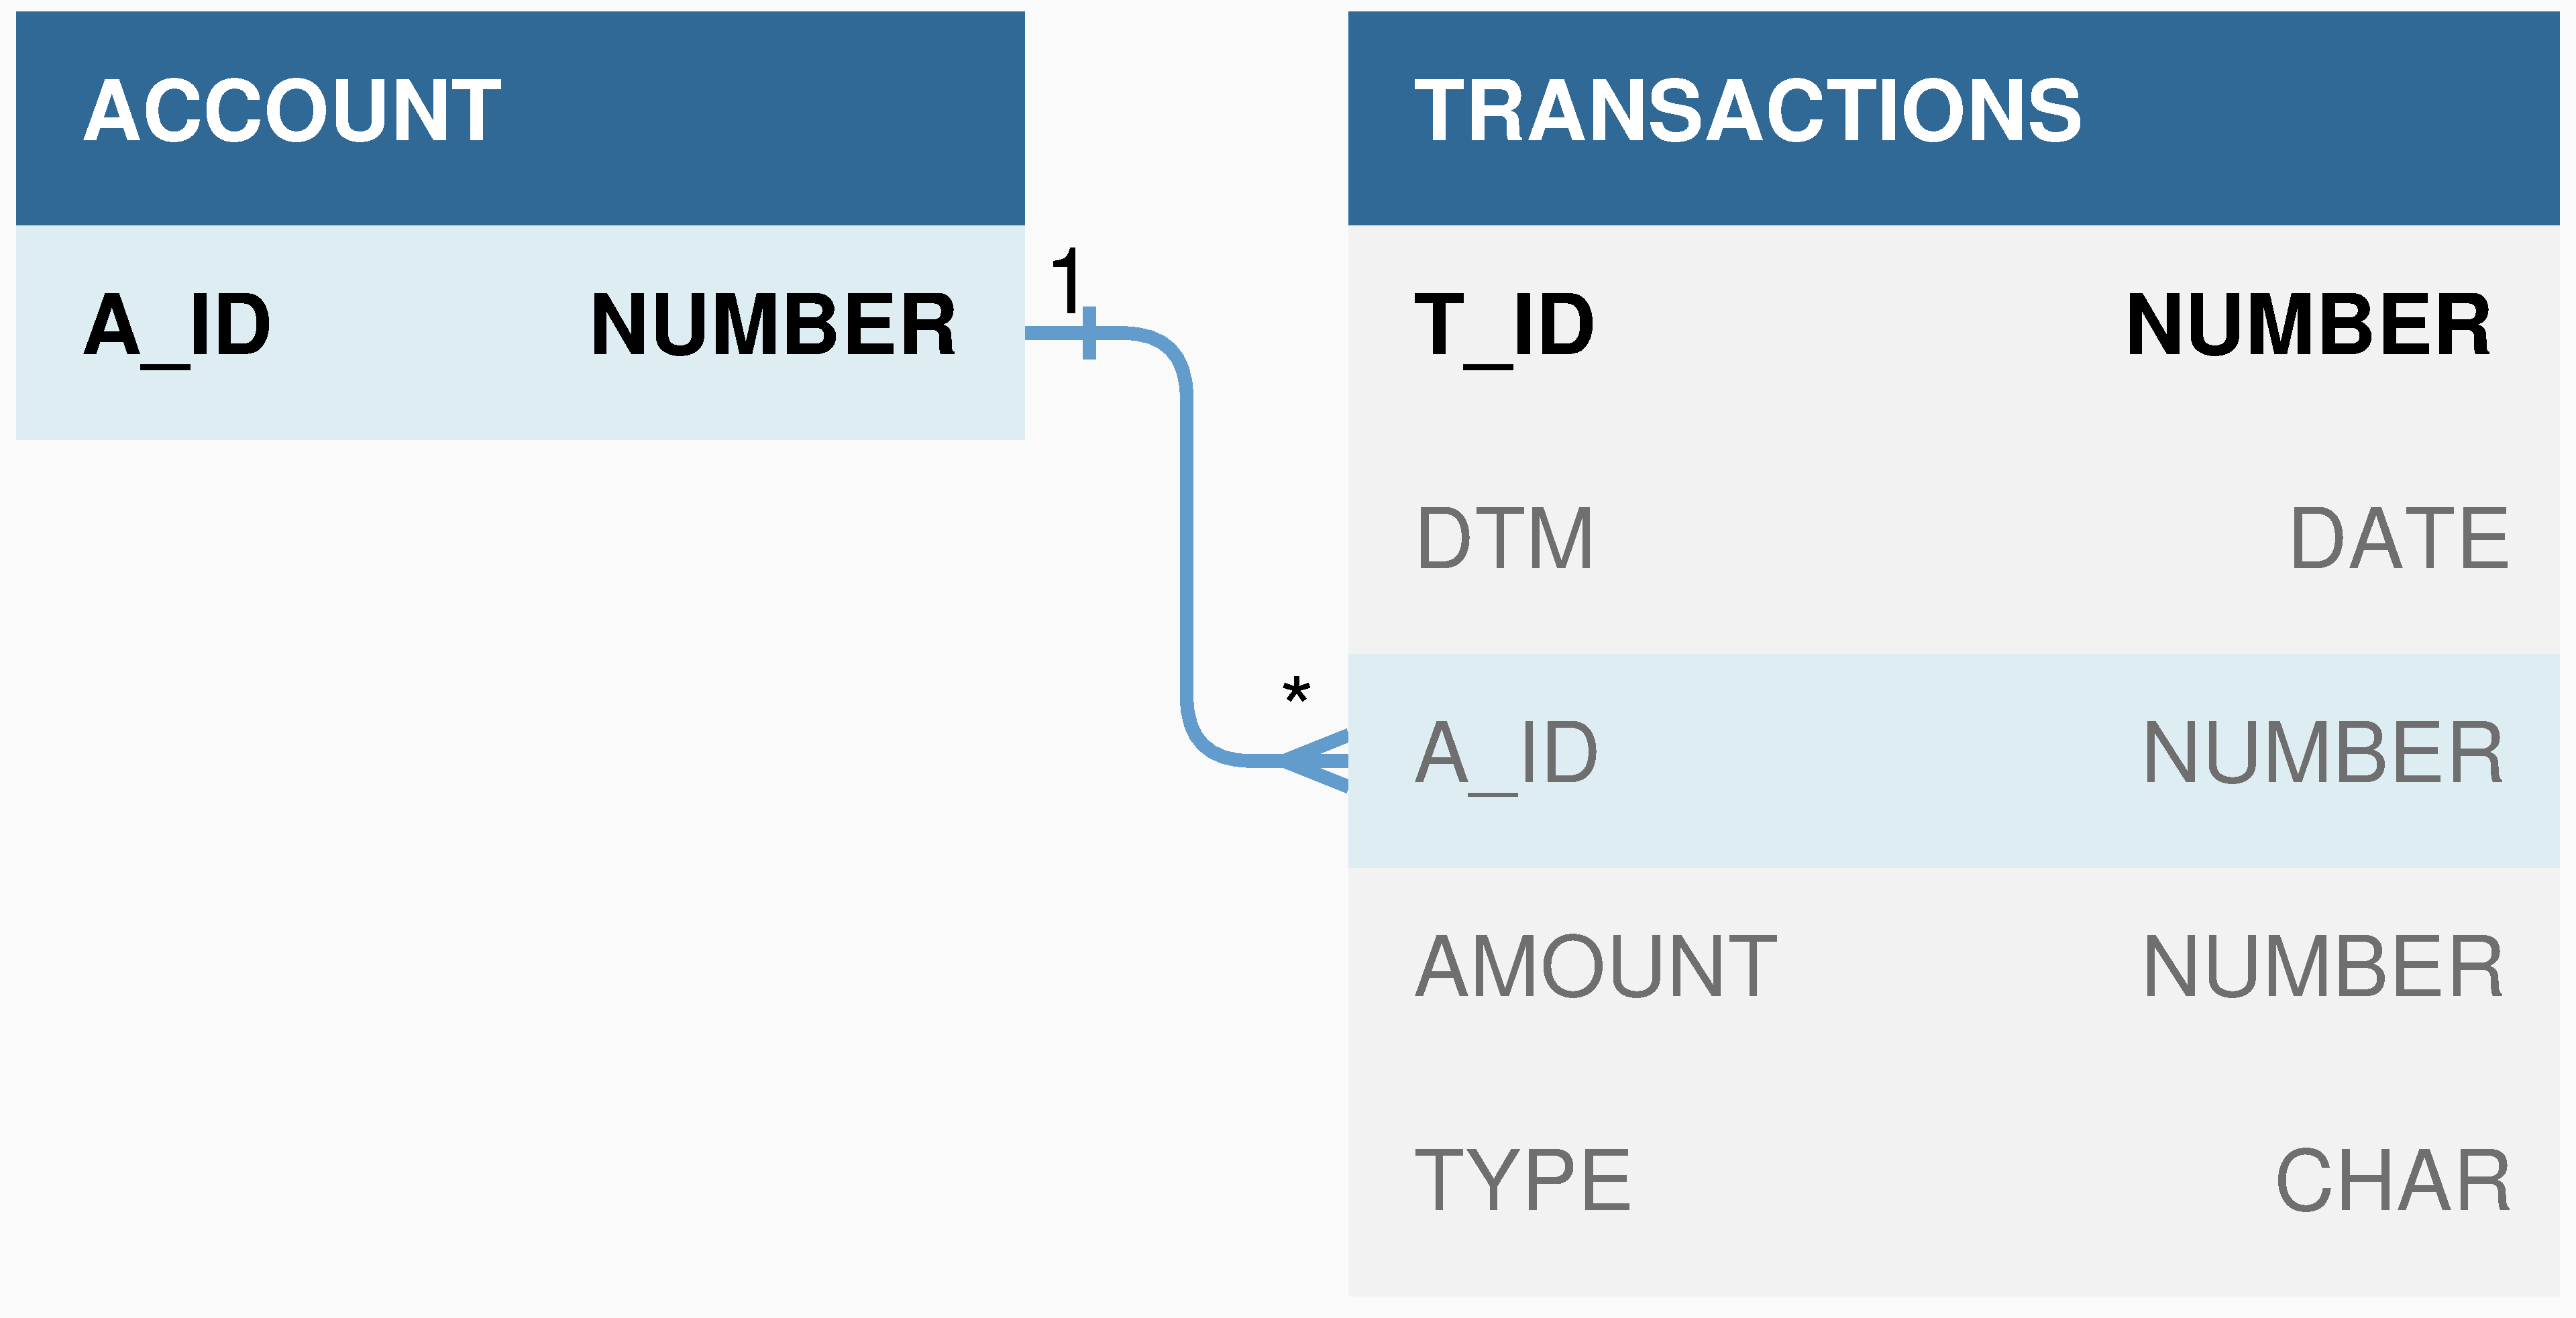
\includegraphics[width=0.5\linewidth]{lab_09_schema.pdf}

\end{figure}
There are 3 types of accounts in the bank:
\begin{enumerate}
    \item \textbf{Commercially Important Person (CIP):} Total transaction volume $> 5,000,000$.
    \item \textbf{Very Important Person (VIP):} Total transaction volume between $2,500,000 - 4,500,000$.
    \item \textbf{Ordinary Person (OP):} Total transaction volume $< 1,000,000$.
\end{enumerate}

\section{Lab Task}
\textbf{First Load the new sql file for the task.} Then write a JAVA code to:
\begin{enumerate}
    \item Count the total number of transactions conducted under account $49$.
    \item Count the number of credit transactions.
    \item List the transactions that occurred in the last 6 months of 2021.
    \item Count the number of CIP, VIP, and OPs. Also show the number of people that do not fall in any of the categories.
    \item \textbf{Safe Insert Task:} Create a Java class that prompts the user for inputs (Account ID, Amount, Type) and inserts a new transaction using a \texttt{PreparedStatement}. Use the current date for the transaction.
\end{enumerate}

% =======================================================
% SECTION: GUIDELINES & SNIPPETS
% =======================================================
\newpage
\section{Useful Syntax \& Coding Guidelines}

Use the following snippets to help you implement the tasks.

\subsection{Retrieving Values from ResultSet}
When iterating through your query results in Java, ensure you match the Java variable type with the database column type.
\begin{lstlisting}[language=Java]
while (result.next()) {
    // Get integer value (e.g., account_id, type)
    int accId = result.getInt("account_id");
    
    // Get decimal/money value
    double amount = result.getDouble("amount");
    
    // Get date value
    Date date = result.getDate("txn_date");
}
\end{lstlisting}

\subsection{Filtering by Date}
For Task 3 (last 6 months of 2021), you can filter directly in your SQL string using the \texttt{WHERE} clause and standard date formats (\texttt{'YYYY-MM-DD'}).
\begin{lstlisting}[language=Java]
String sqlQuery = "SELECT * FROM transactions " +
                  "WHERE txn_date >= '2021-07-01' " +
                  "AND txn_date <= '2021-12-31'";
\end{lstlisting}

\subsection{Calculating Balance \& Volume}
Since the \texttt{ACCOUNT} table does not store the balance, you must calculate it by fetching all transactions for a specific user and processing them in Java.

\begin{itemize}
    \item \textbf{Balance:} Start at 0. Add \texttt{amount} if \texttt{type == 0} (Credit). Subtract \texttt{amount} if \texttt{type == 1} (Debit).
    \item \textbf{Volume:} Sum of all \texttt{amount}s, regardless of type.
\end{itemize}

\begin{lstlisting}[language=Java]
double balance = 0;
double totalVolume = 0;

if (type == 0) { // Credit
    balance += amount;
} else if (type == 1) { // Debit
    balance -= amount;
}
totalVolume += amount;
\end{lstlisting}

\subsection{PreparedStatement Syntax}
To solve the safe insert task, you must use \texttt{?} placeholders instead of concatenating strings.

\begin{lstlisting}[language=Java]
// 1. Write SQL with placeholders
String insertSQL = "INSERT INTO transactions (txn_date, a_id, amount, type) VALUES (?, ?, ?, ?)";

// 2. Create PreparedStatement
PreparedStatement pstmt = con.prepareStatement(insertSQL);

// 3. Fill the placeholders (Index starts at 1)
// Example: Setting the date to today
long millis = System.currentTimeMillis();
pstmt.setDate(1, new java.sql.Date(millis)); 

// Example: Setting the Account ID (e.g., from user input)
pstmt.setInt(2, 49); 

// Example: Setting the Amount and Type
pstmt.setDouble(3, 500.00); 
pstmt.setInt(4, 0); 

// 4. Execute the Insert
pstmt.executeUpdate();
\end{lstlisting}


% =======================================================
% SECTION: PYTHON POSTGRES
% =======================================================
\newpage
\section{PostgreSQL in Python}

While this lab focuses on Java (JDBC), real-world applications often use Python for database interaction, especially in Data Science and Web Development (e.g., Django, Flask). 

In Python, the most popular driver is \texttt{psycopg2}. The logic remains very similar to JDBC: you need a Connection, a Cursor (similar to Statement), and you Execute queries.

\subsection{1. Installation}
Unlike Java where you add a JAR file, in Python you install the package via terminal:
\begin{lstlisting}[language=bash]
pip install psycopg2-binary
\end{lstlisting}

\subsection{2. Python Code Example}
This script connects to the same \texttt{cse4308\_12345} database (as user \texttt{student\_12345}) you created earlier.

\begin{lstlisting}[language=Python]
import psycopg2

try:
    # 1. Establish Connection
    connection = psycopg2.connect(
        user="student_12345",
        password="student12345",
        host="localhost",
        port="5432",
        database="cse4308_12345"
    )

    # 2. Create Cursor (Similar to JDBC Statement)
    cursor = connection.cursor()

    # 3. Execute Query
    cursor.execute("SELECT * FROM account LIMIT 5;")

    # 4. Fetch Results (Similar to ResultSet)
    records = cursor.fetchall()
    
    print("Printing first 5 accounts:")
    for row in records:
        print("Account ID:", row[0])

except (Exception, psycopg2.Error) as error:
    print("Error while connecting to PostgreSQL", error)

finally:
    # 5. Close Connection
    if connection:
        cursor.close()
        connection.close()
        print("PostgreSQL connection is closed")
\end{lstlisting}

% =======================================================
% SUBMISSION GUIDELINES
% =======================================================
\end{document}